\documentclass{beamer}
\usepackage[english]{babel}
\usepackage[utf8]{inputenc}
\mode<presentation>{\usetheme{FS18}}
\usepackage{amsmath,amsthm, amssymb, latexsym}
\usepackage[orientation=portrait,size=a0,scale=1.4]{beamerposter}
\usepackage{natbib}
\graphicspath{{../figures/graphics/}}
 
\title{A Continuous-Time Dynamical System Describing both Rate Encoding and Spiking Neurons}
\author{Fabian Schubert, Claudius Gros}
\institute{Institute for Theoretical Physics, Goethe University Frankfurt a.M.}
\date[Feb. 28th, 2018]{Feb. 28th, 2018}


\begin{document}
\begin{frame}[t]
\begin{columns}[t]
\begin{column}{.45\textwidth}

\begin{myblock}{Introduction}
\begin{itemize}
\item We investigated a two-dimensional nonlinear system, modeling a wide range of dynamic 
properties of spiking neurons.
\item By altering key parameters of this system, its dynamics become identical to those of a 
time-continuous rate-encoding model.
\item Differences of the dynamical properties of single units as well as of network structures under 
these two regimes can be treated within the same mathematical framework.
\end{itemize}
\end{myblock}

\begin{myblock}{Neuron Model}
\begin{itemize}
\item The model consists of a two-dimensional non-linear system given by
\end{itemize}
\begin{minipage}[t]{.5\linewidth}
\begin{align*}
\tau_x \dot{x} &= f(x) - y  \\ 
\tau_y \dot{y} &= g(x) - y \\
u(x,y) &:= \frac{x+y}{\sqrt{2}}
\end{align*}
\end{minipage}%
\begin{minipage}[t]{.5\linewidth}
\begin{align*}
f(x) &= s \sigma \left(a\left(x-s/4\right)\right)  \\
g(x) &= g_0 \sigma\left(a_g\left(x-I\right)\right) - \Delta_y \\
\sigma(x) &= \left(1+\mathrm{exp}(-x)\right)^{-1}
\end{align*}
\end{minipage}
\begin{figure}
\centering
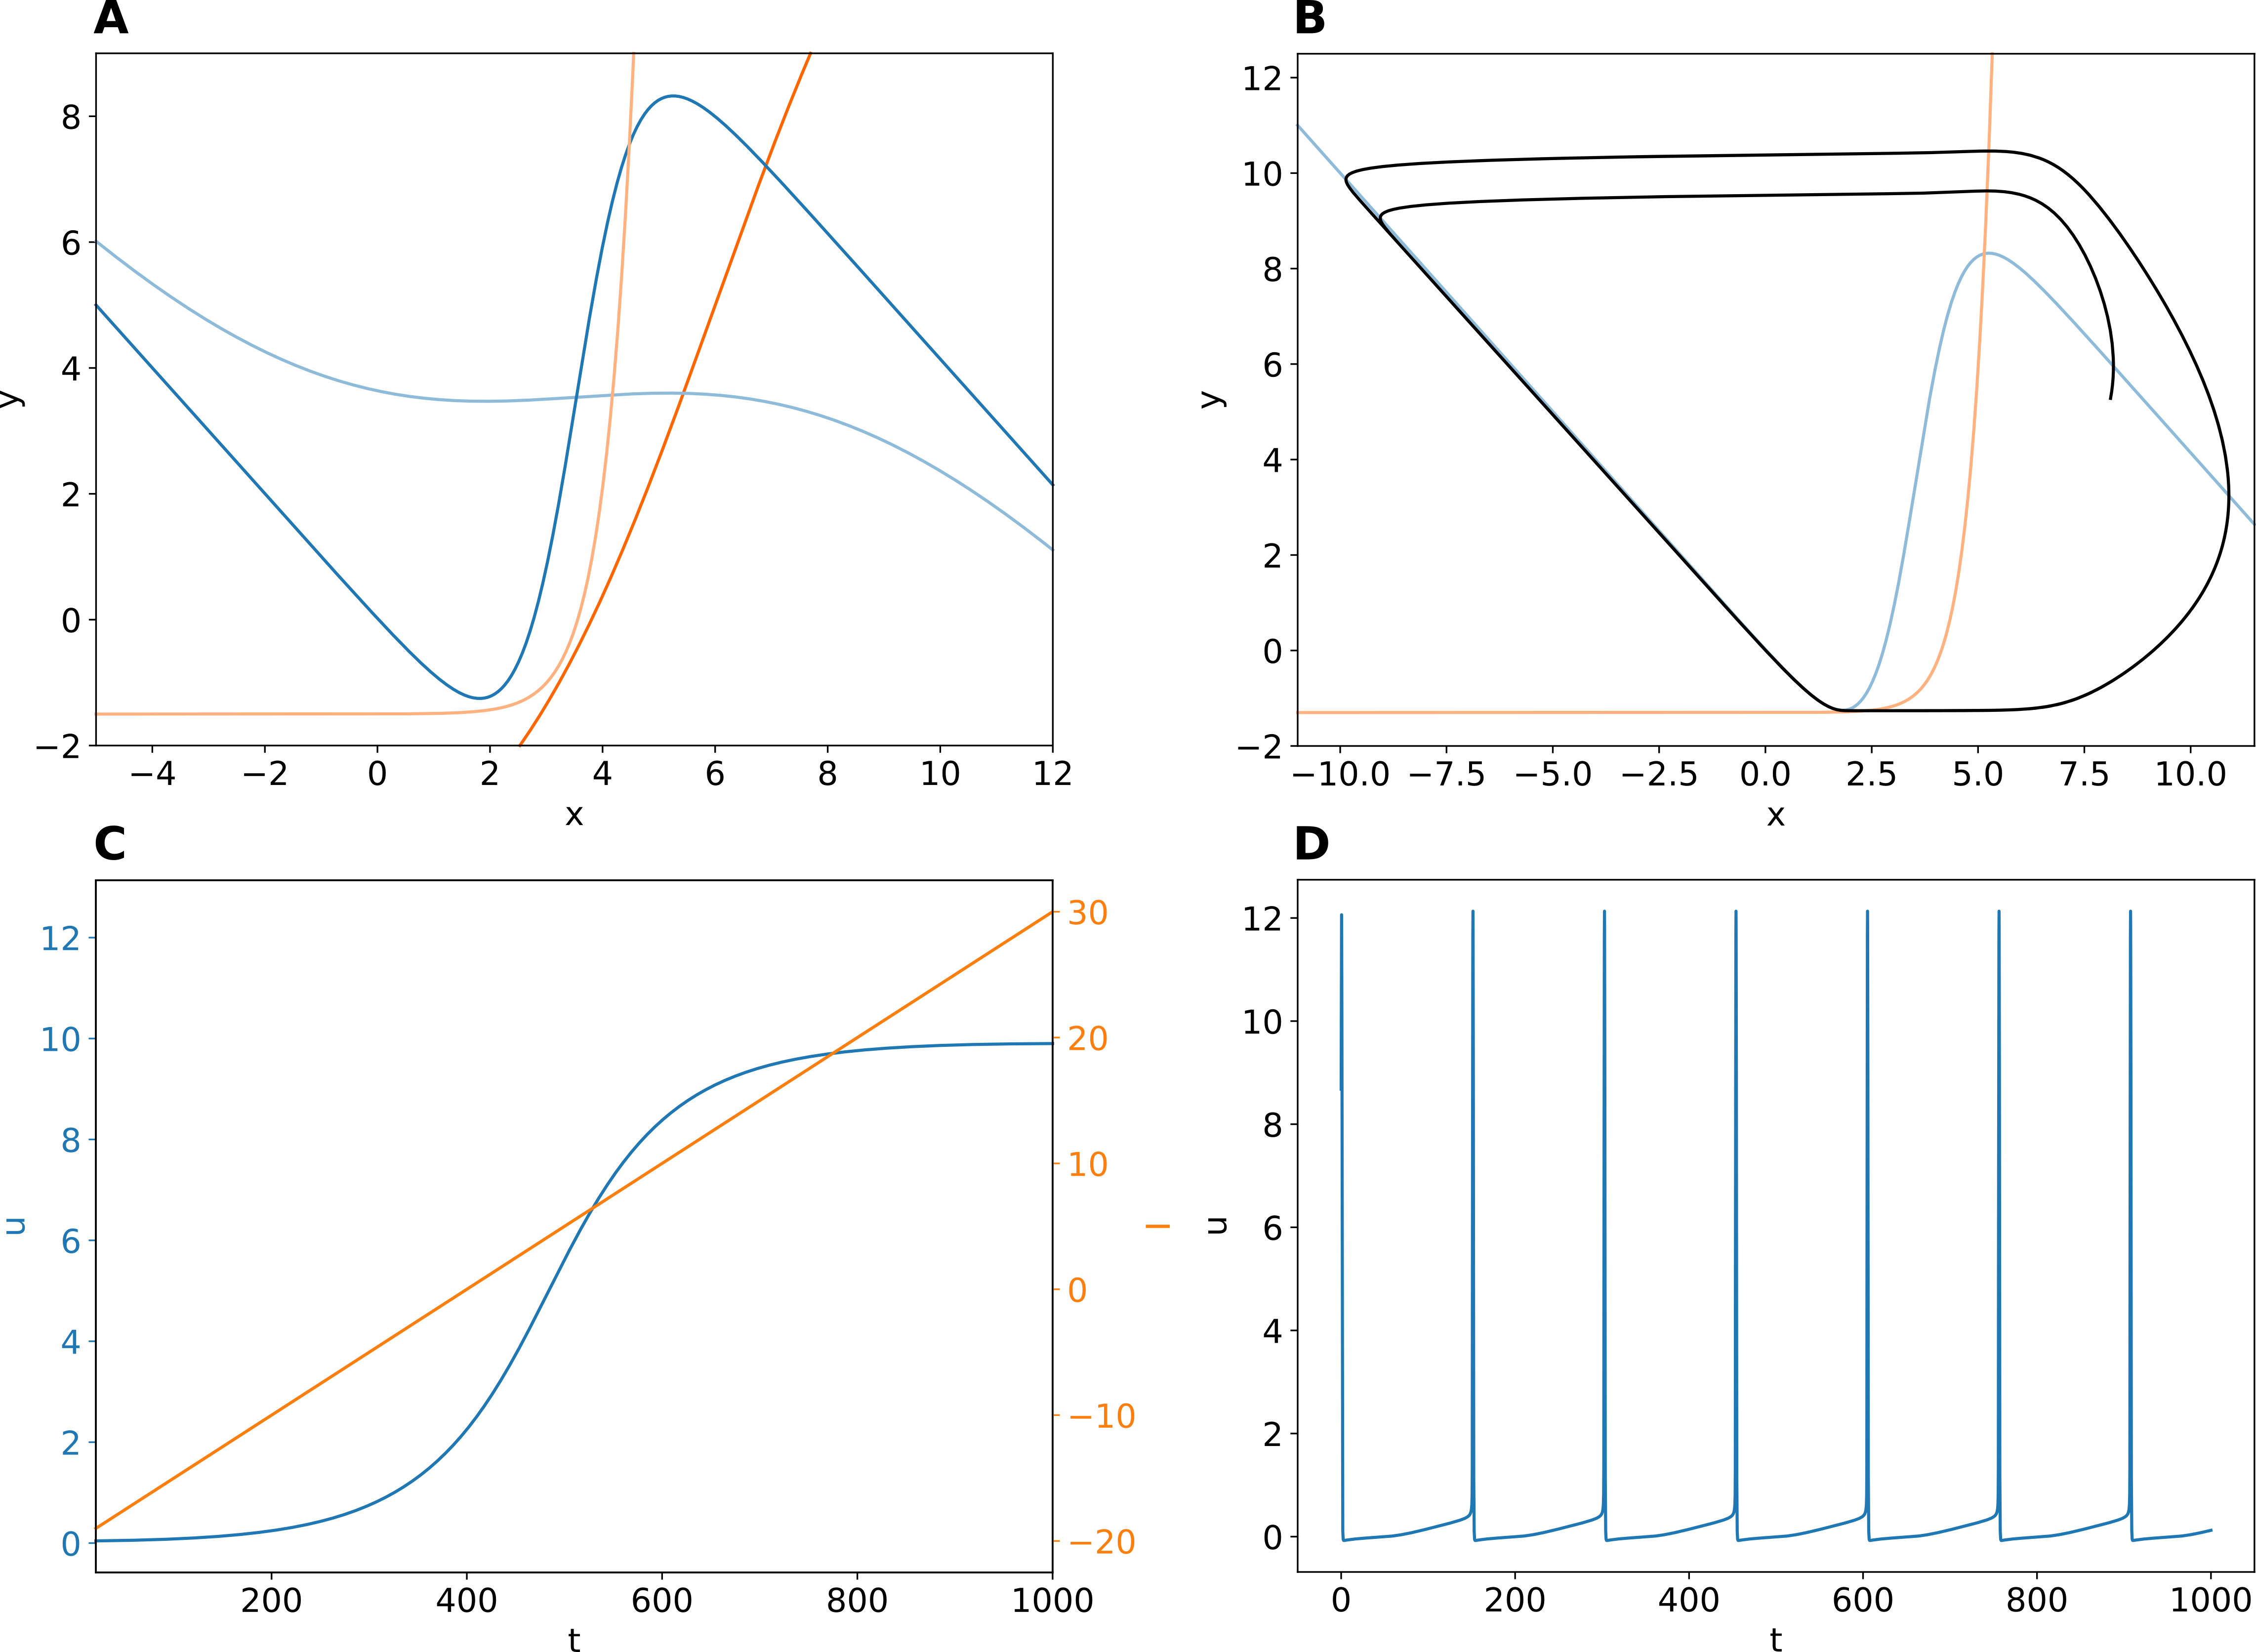
\includegraphics[width=0.8\textwidth]{../figures/graphics/dynamics_combined_figure.png}
\caption{\textbf{A}: x/y-nullclines (blue/red) of the dynamical system for parameter sets generating spiking/non spiking behavior. \textbf{B}: Phase plane trajectory for the spiking dynamics. \textbf{C}/\textbf{D}: Dynamics of readout variable $u$ for the spiking/non-spiking case.}
\label{fig:dynamics_illustr}
\end{figure}
\end{myblock}

\begin{myblock}{Spiking Neuron Model}
\begin{itemize}
\item A range of different types of spiking dynamics can be reproduced by this generic system.
\end{itemize}
\begin{figure}
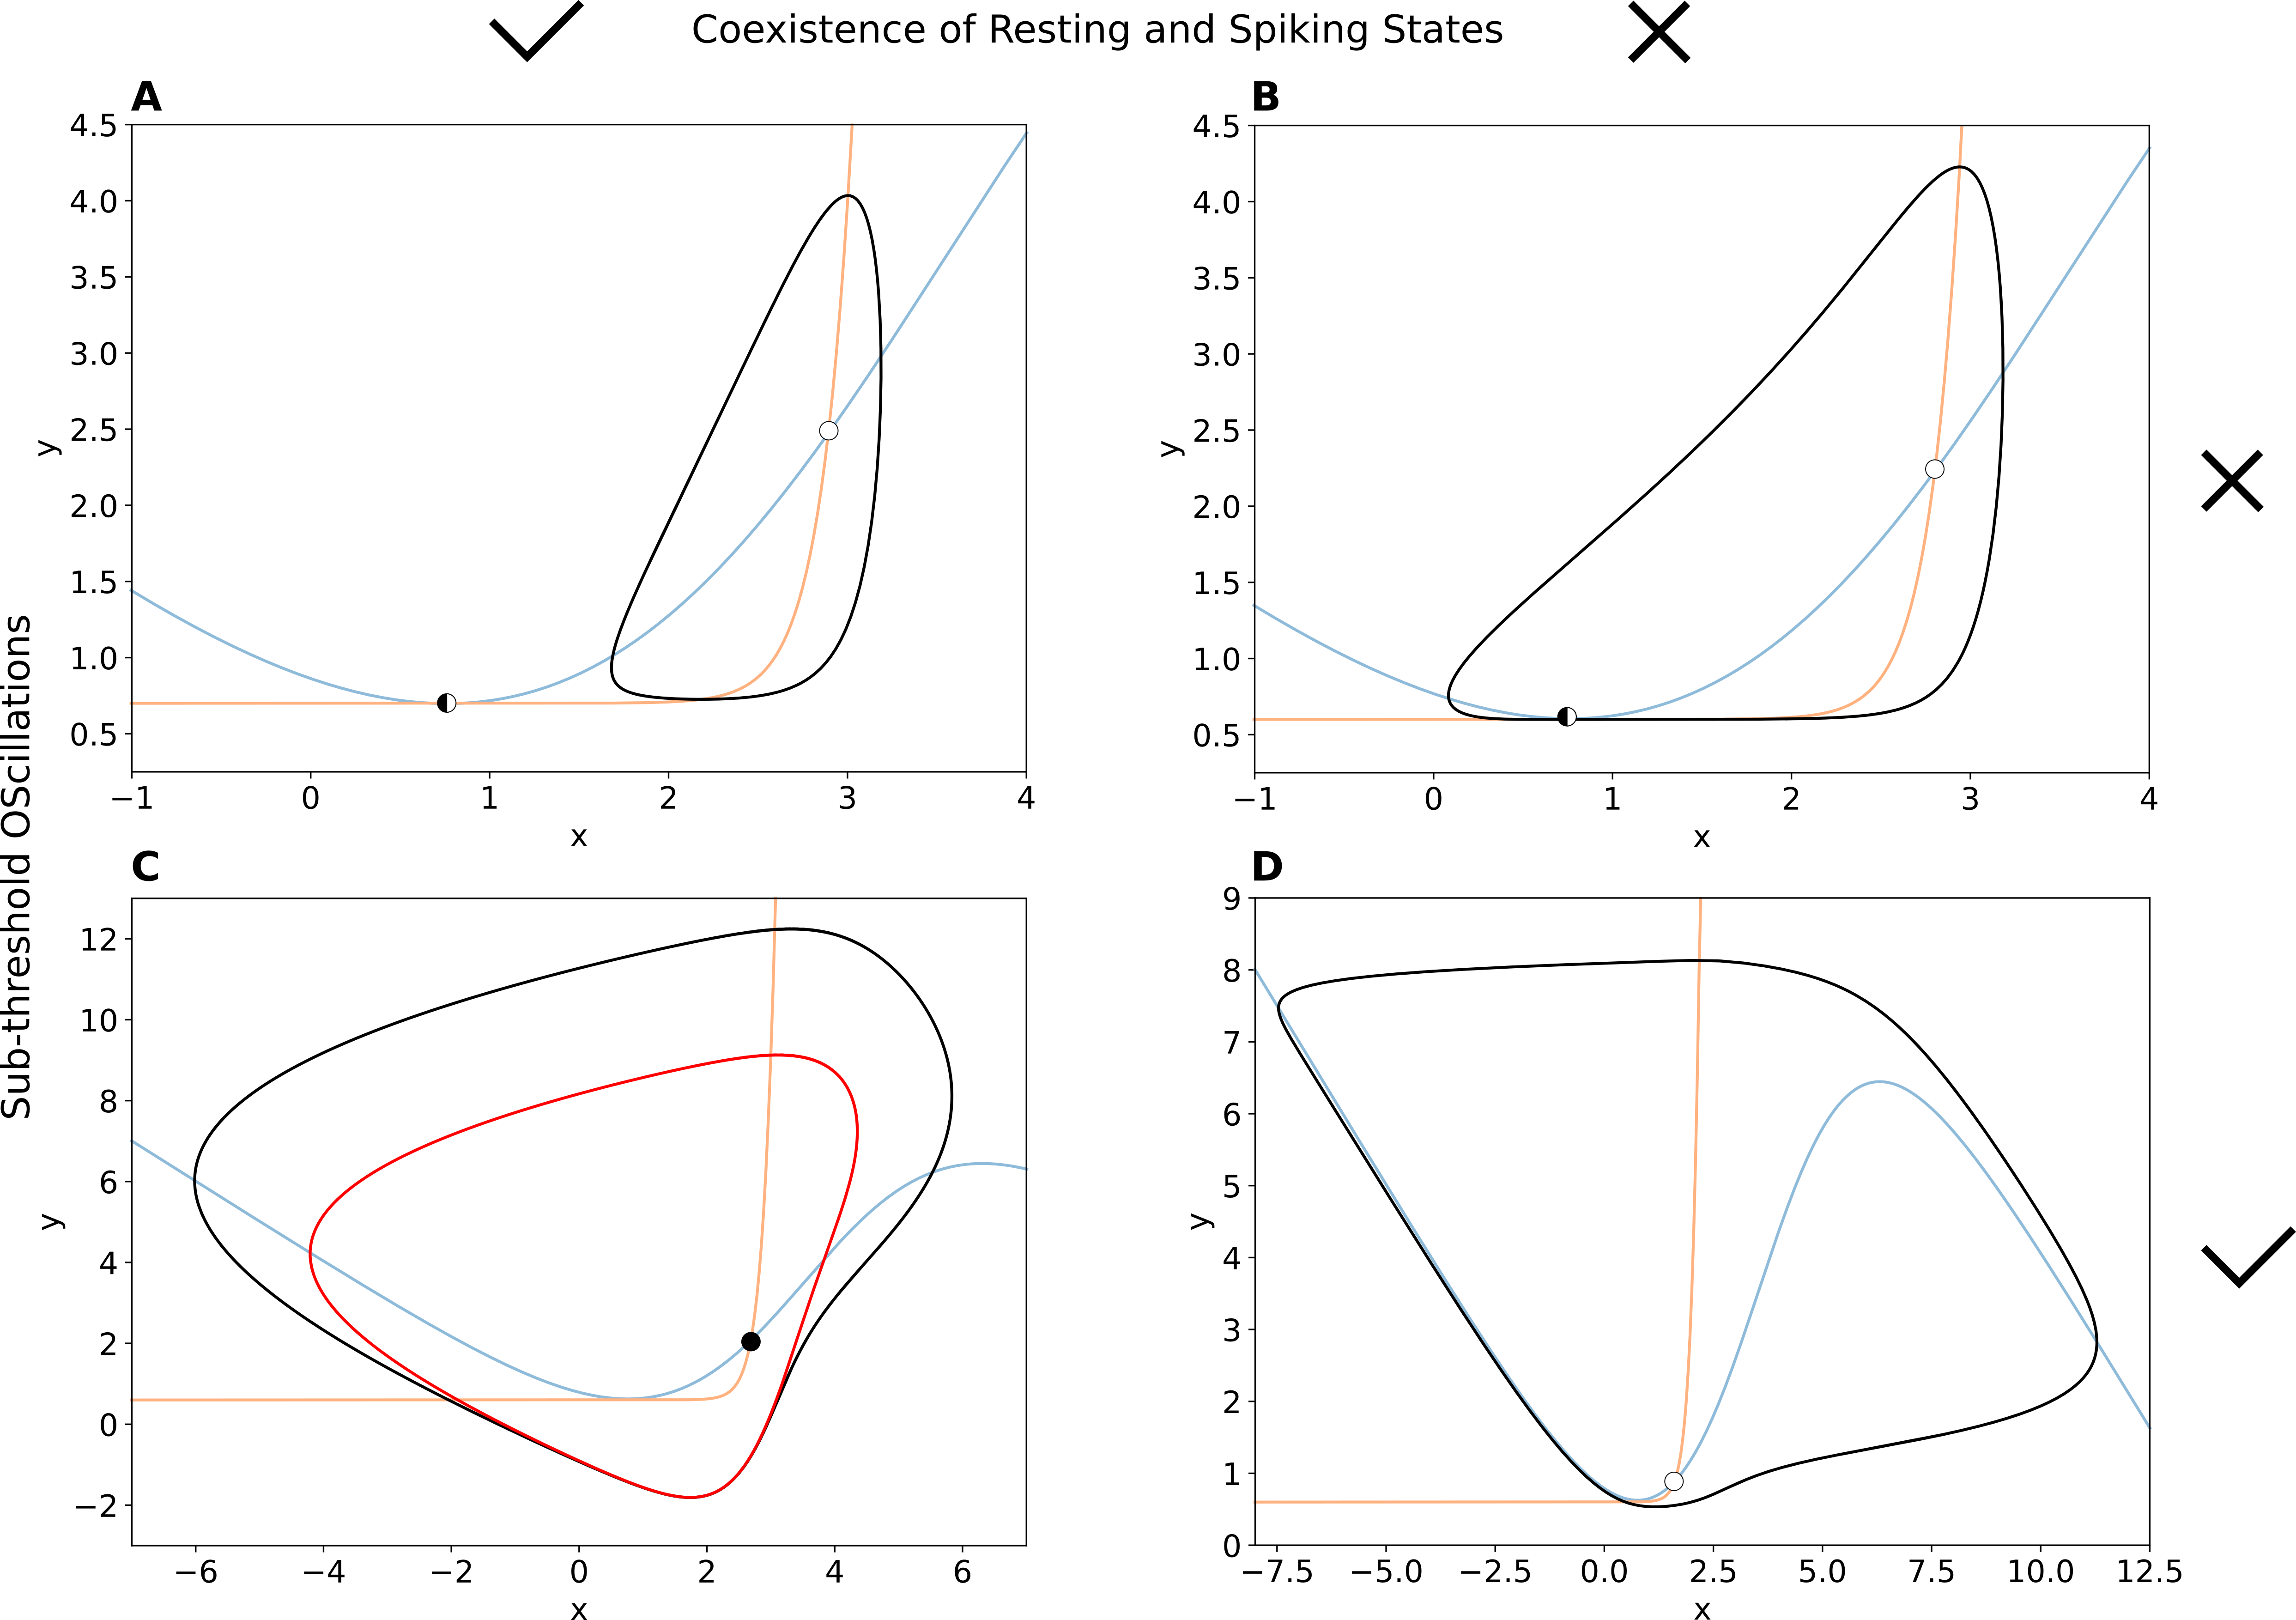
\includegraphics[width=0.8\textwidth]{../figures/graphics/bif_types_combined_figure.png}
\caption{Examples of spiking dynamics/bifurcations observed in the model, ordered by the property of coexistence of resting/spiking states and the possibility of sub-threshold oscillations. A: Saddle node bifurcation with coexisting limit cycle. B: Saddle node b. on invariant cycle. C: Subcritical Hopf b/ Fold b. of limit cycles. C: Supercritical Hopf b.}
\label{fig:bif_types_combined}
\end{figure}
\begin{itemize}
\item Based on the classification by Izhikevich \cite{Izhikevich_2007}, our model was able to generate class 1 (arbitrary small firing rates) as well as class 2 (all-or-none spiking behavior) firing patterns.
\item Due to the relatively simple mathematical form of our system, we could perform analytical analyses and predictions about firing behavior closely matching the simulation results, see Fig. \ref{fig:saddle_bif_fir_rates}.
\end{itemize}
\begin{figure}
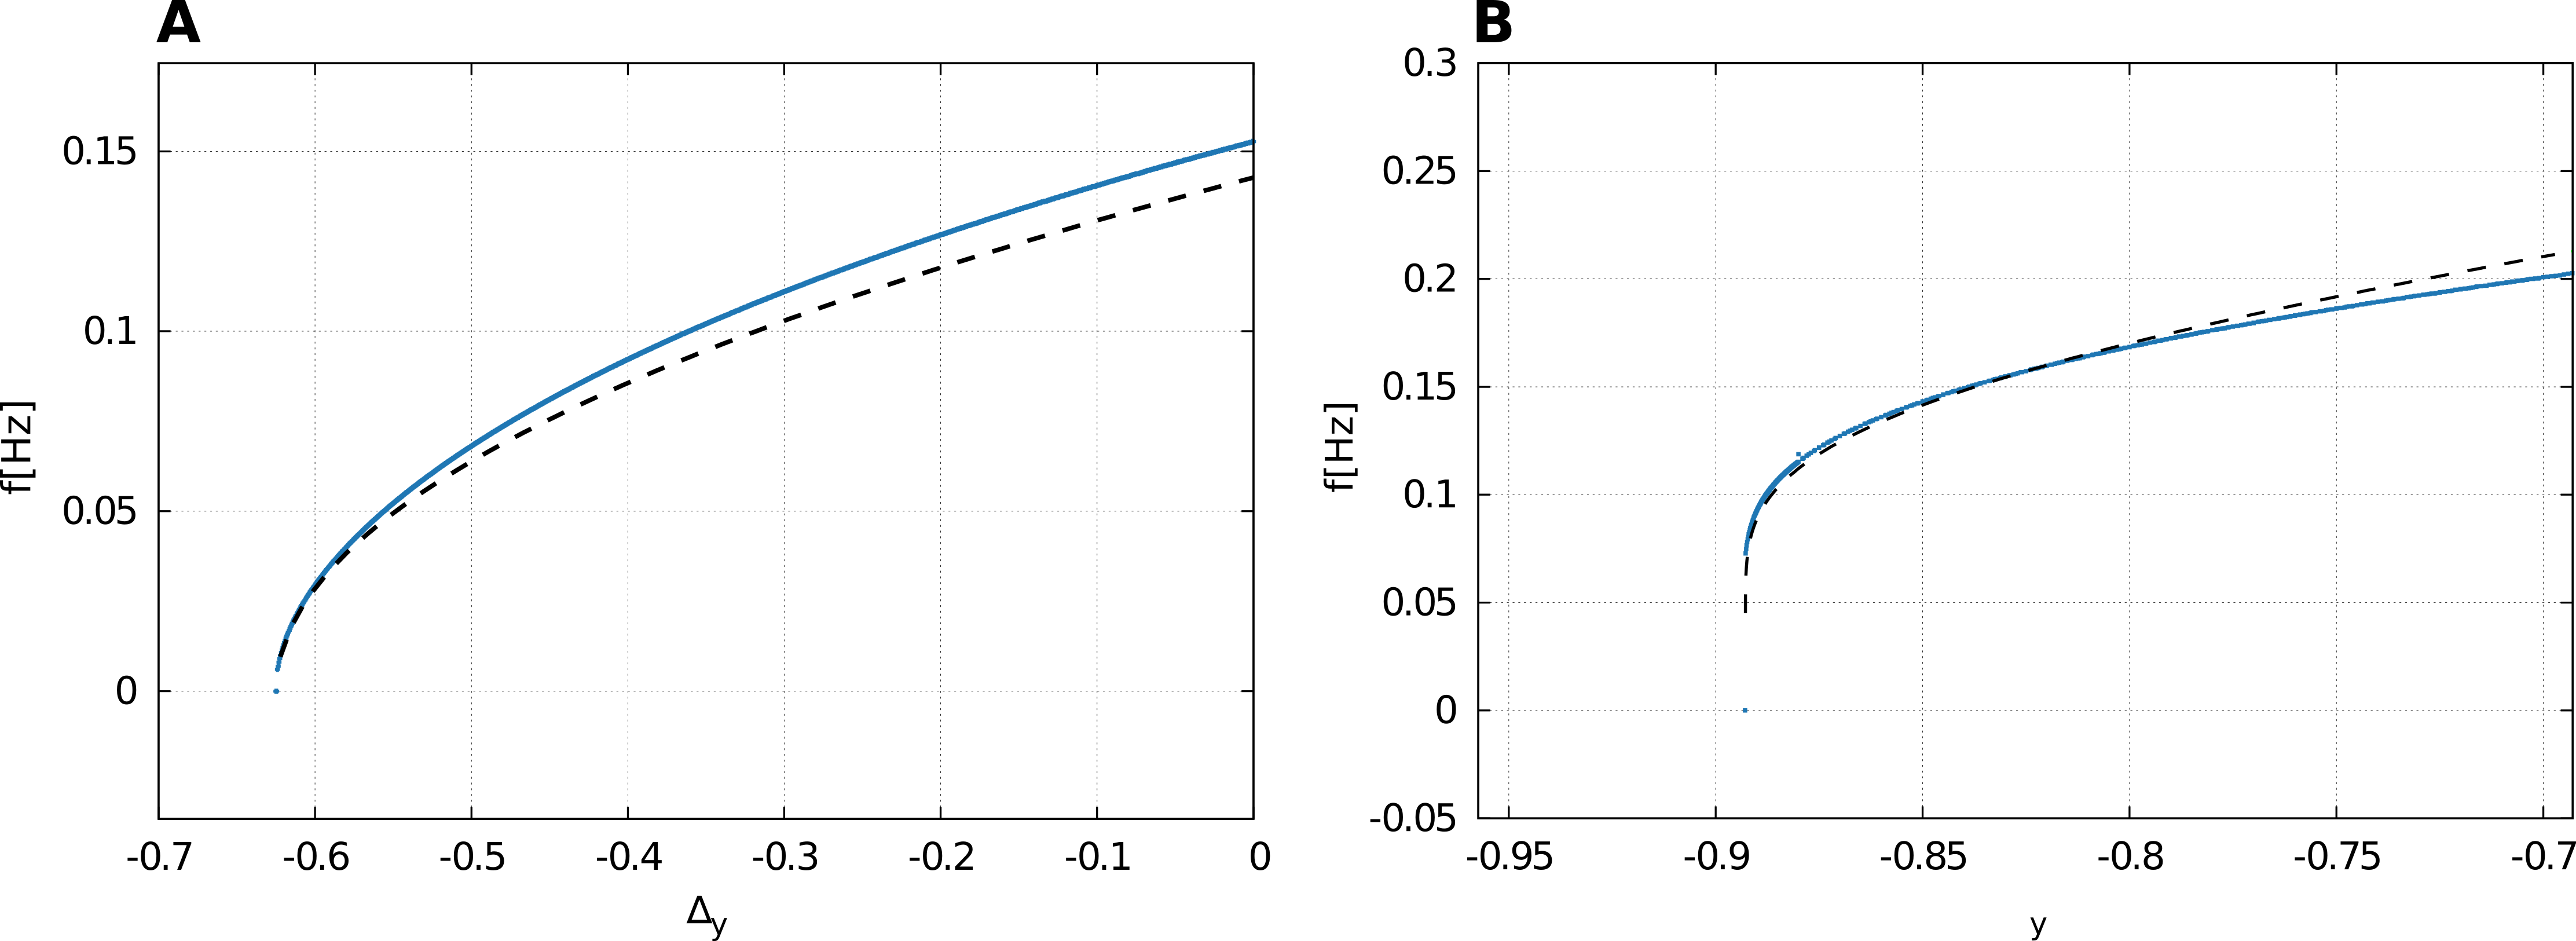
\includegraphics[width=0.8\textwidth]{../figures/graphics/saddle_bif_fir_rates_combined.png}
\caption{Measured and predicted firing rates as a function of $\Delta_y$ under the configurations shown in Fig. \ref{fig:bif_types_combined}A/B.}
\label{fig:saddle_bif_fir_rates}
\end{figure}
\end{myblock}
\end{column}
\begin{column}{.45\textwidth}

\begin{myblock}{Fitting Experimental Data}
\begin{figure}
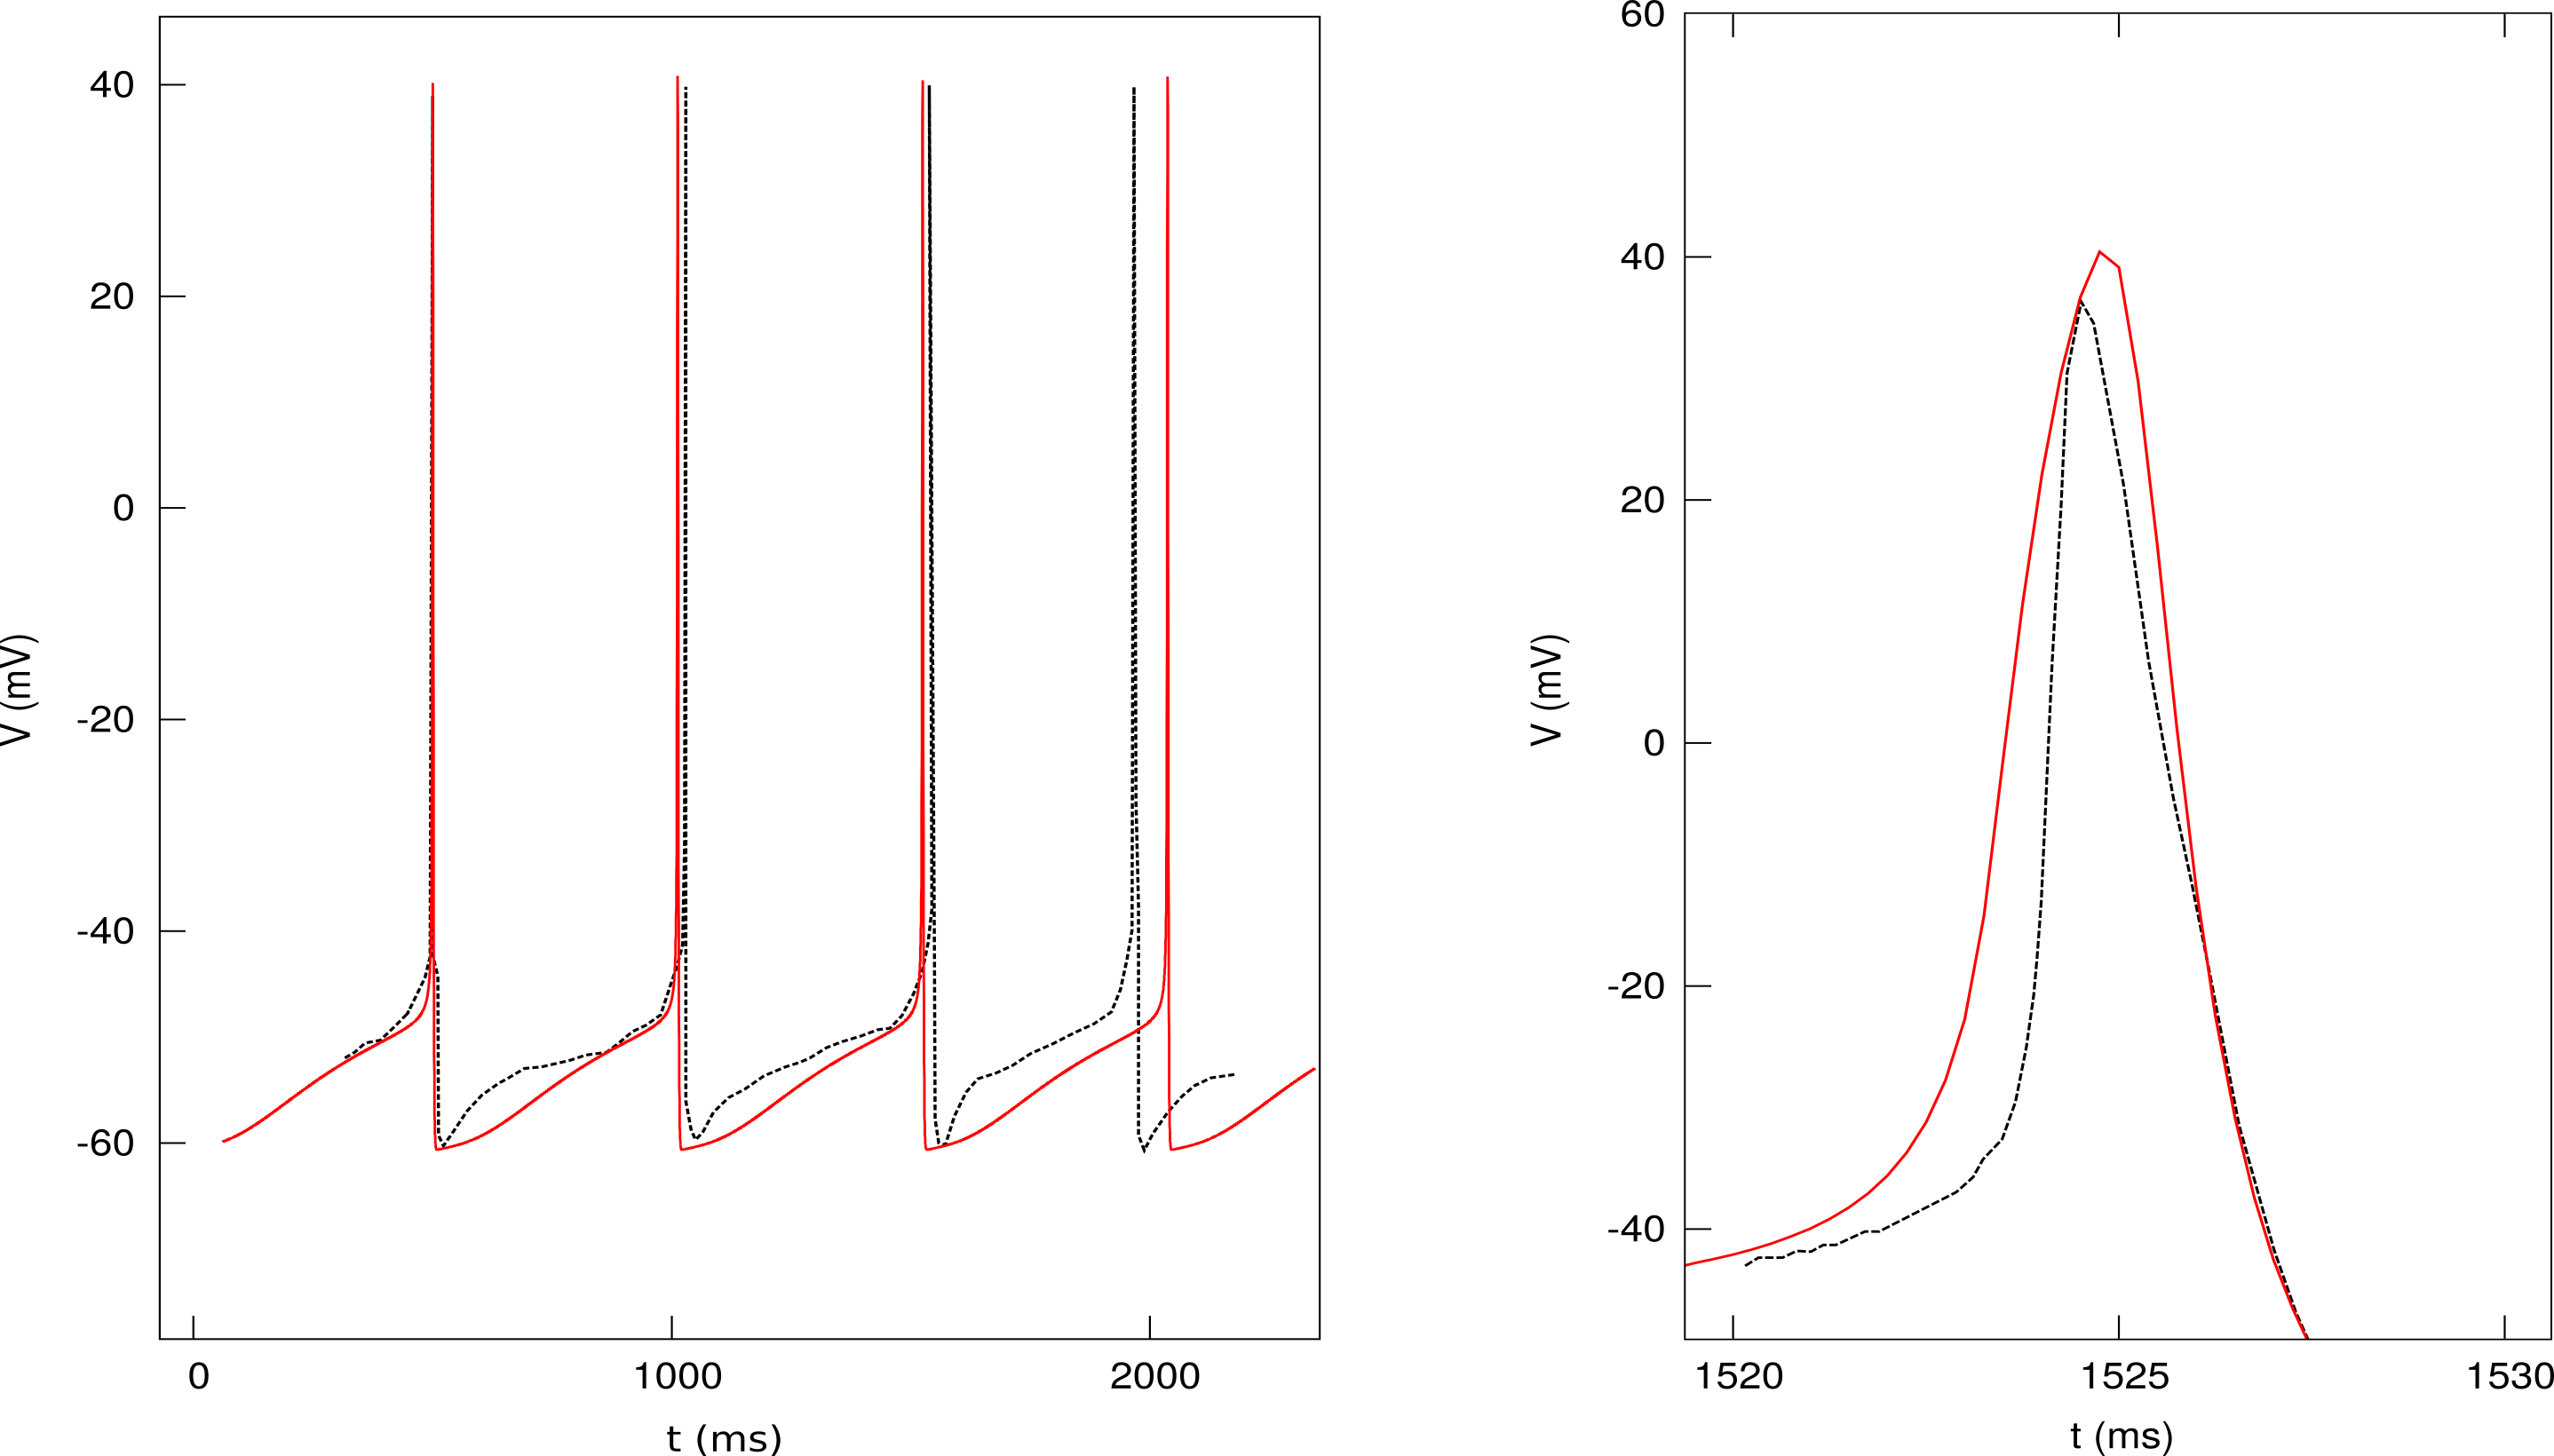
\includegraphics[width=0.7\textwidth]{../figures/graphics/spikefit.png}
\caption{Fit of the dynamical system onto measurements of a dopaminergic
neuron in the Substantia Nigra of a mouse brain \cite{Bean_2007}.}
\label{fig:spikefit}
\end{figure}
\begin{itemize}
\item The parameters of the dynamical systems allow to easily control key features of the voltage trace, such as spike height, spike width and threshold potential.
\end{itemize}
\begin{align*}
u_{\rm spike height} &\approx s/\sqrt{2} \\
\Delta t_{\rm spike} &\propto g_O^{-1} \\
u_{\rm threshold} &\approx 1/\sqrt{2a}
\end{align*}
\end{myblock}

\begin{myblock}{Rate Encoding Model}
\begin{itemize}
\item The system's parameters can be tuned such that dynamics transition from a spiking behavior to a relaxation towards an input-dependent fixed point.
\item The projection of this fixed point onto $u$ follows a sigmoidal as input increases, see Fig. \ref{fig:dynamics_illustr}C.  
\end{itemize}
\begin{figure}
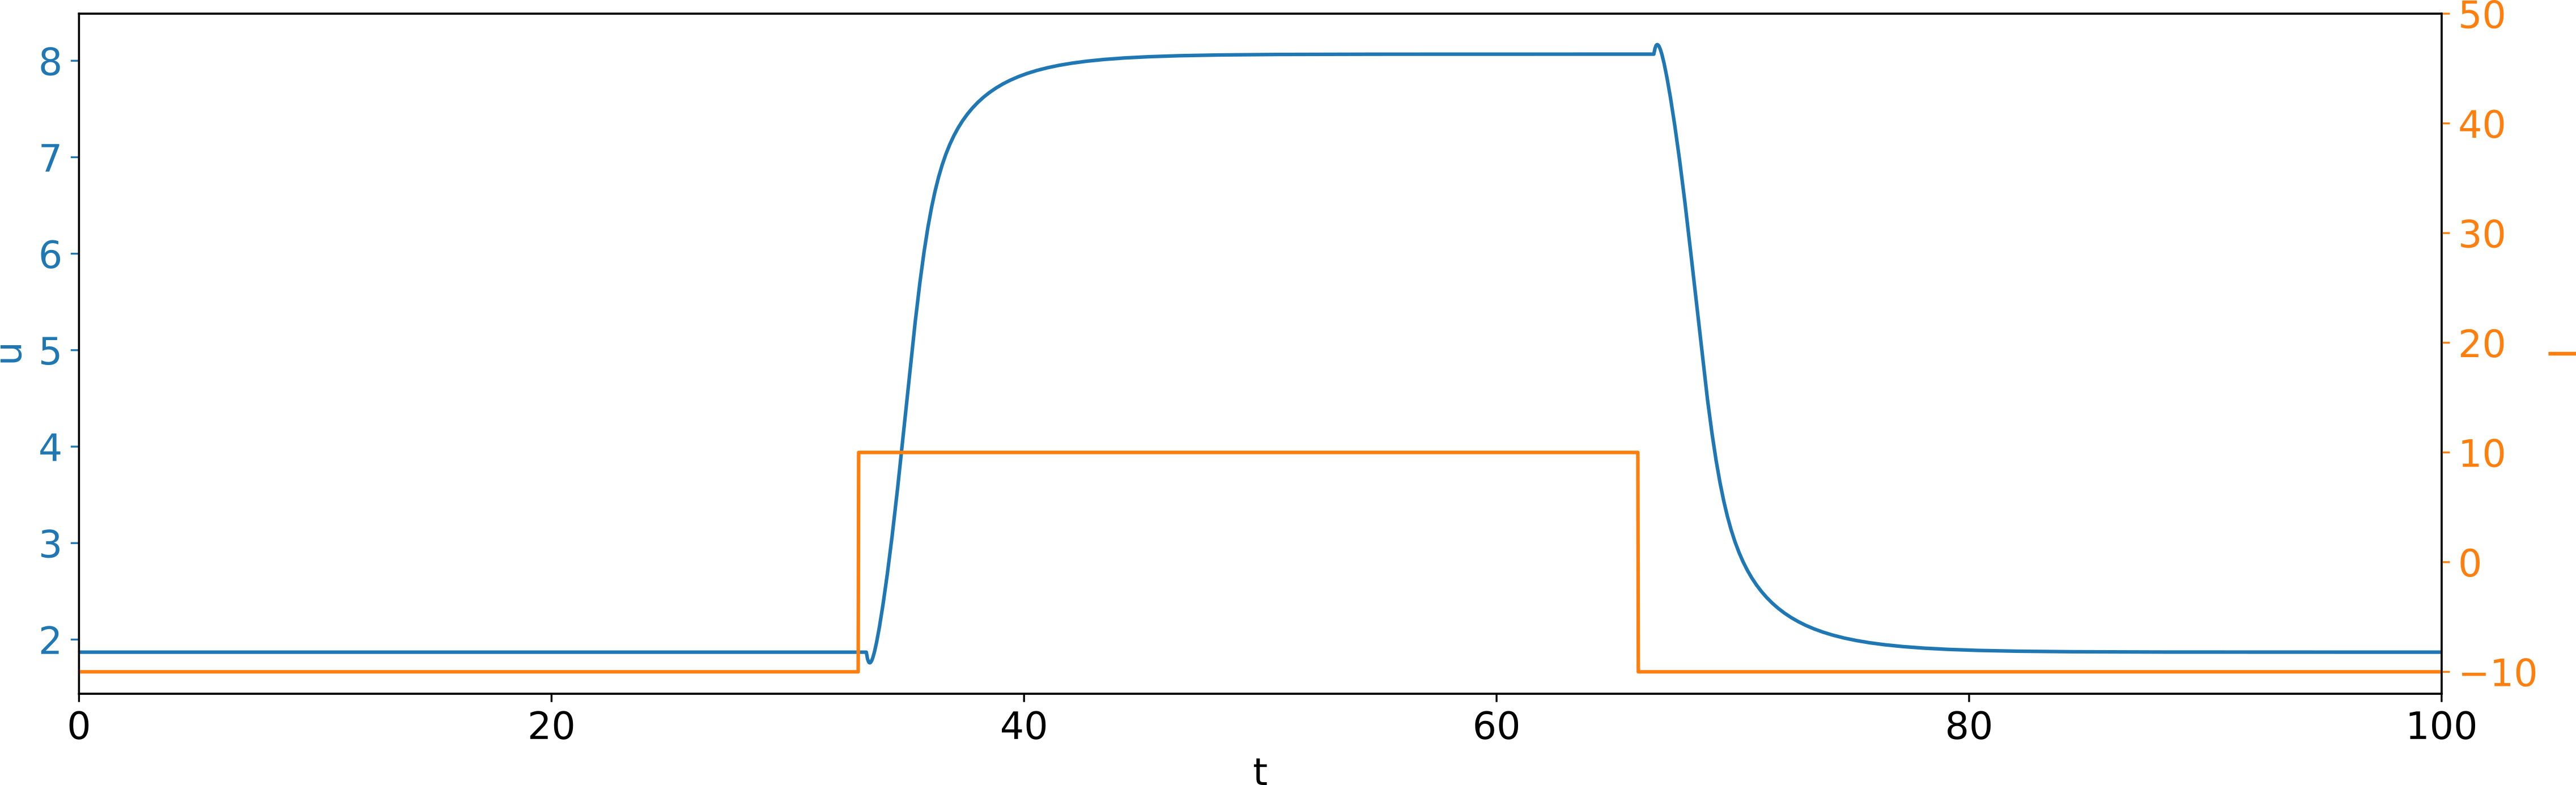
\includegraphics[width=0.9\textwidth]{../figures/graphics/rate_dyn_u_step_illustr.png}
\caption{Rate-dynamics response of the readout variable $u$ upon external step input.}
\label{fig:rate_dyn_u_step}
\end{figure}
\begin{itemize}
\item The dynamics of $u$ approximately follow those of 1d-system of the form $\tau \dot{u} = -u + \frac{s}{\sqrt{2}}\sigma\left( c \cdot I\right)$. The time constant $\tau$ is then described by $\tau = -\frac{1}{\langle \lambda \rangle}$, where $\langle \lambda \rangle$ is the mean of the eigenvalues of the fixed point's Jacobian.
\end{itemize}
\end{myblock}

\begin{myblock}{Usage in Networks}
\begin{itemize}
\item Combining our model with a simple model of synaptic transmission resulted in stable network dynamics for both spiking and rate encoding dynamics.
\end{itemize}
\begin{align*}
\tau_g \dot{g} &= -g + w \cdot u_{\rm pre} \\
I_{\rm syn} &= g(E_{\rm syn,exc/inh} - u_{\rm post})
\end{align*}
\begin{figure}
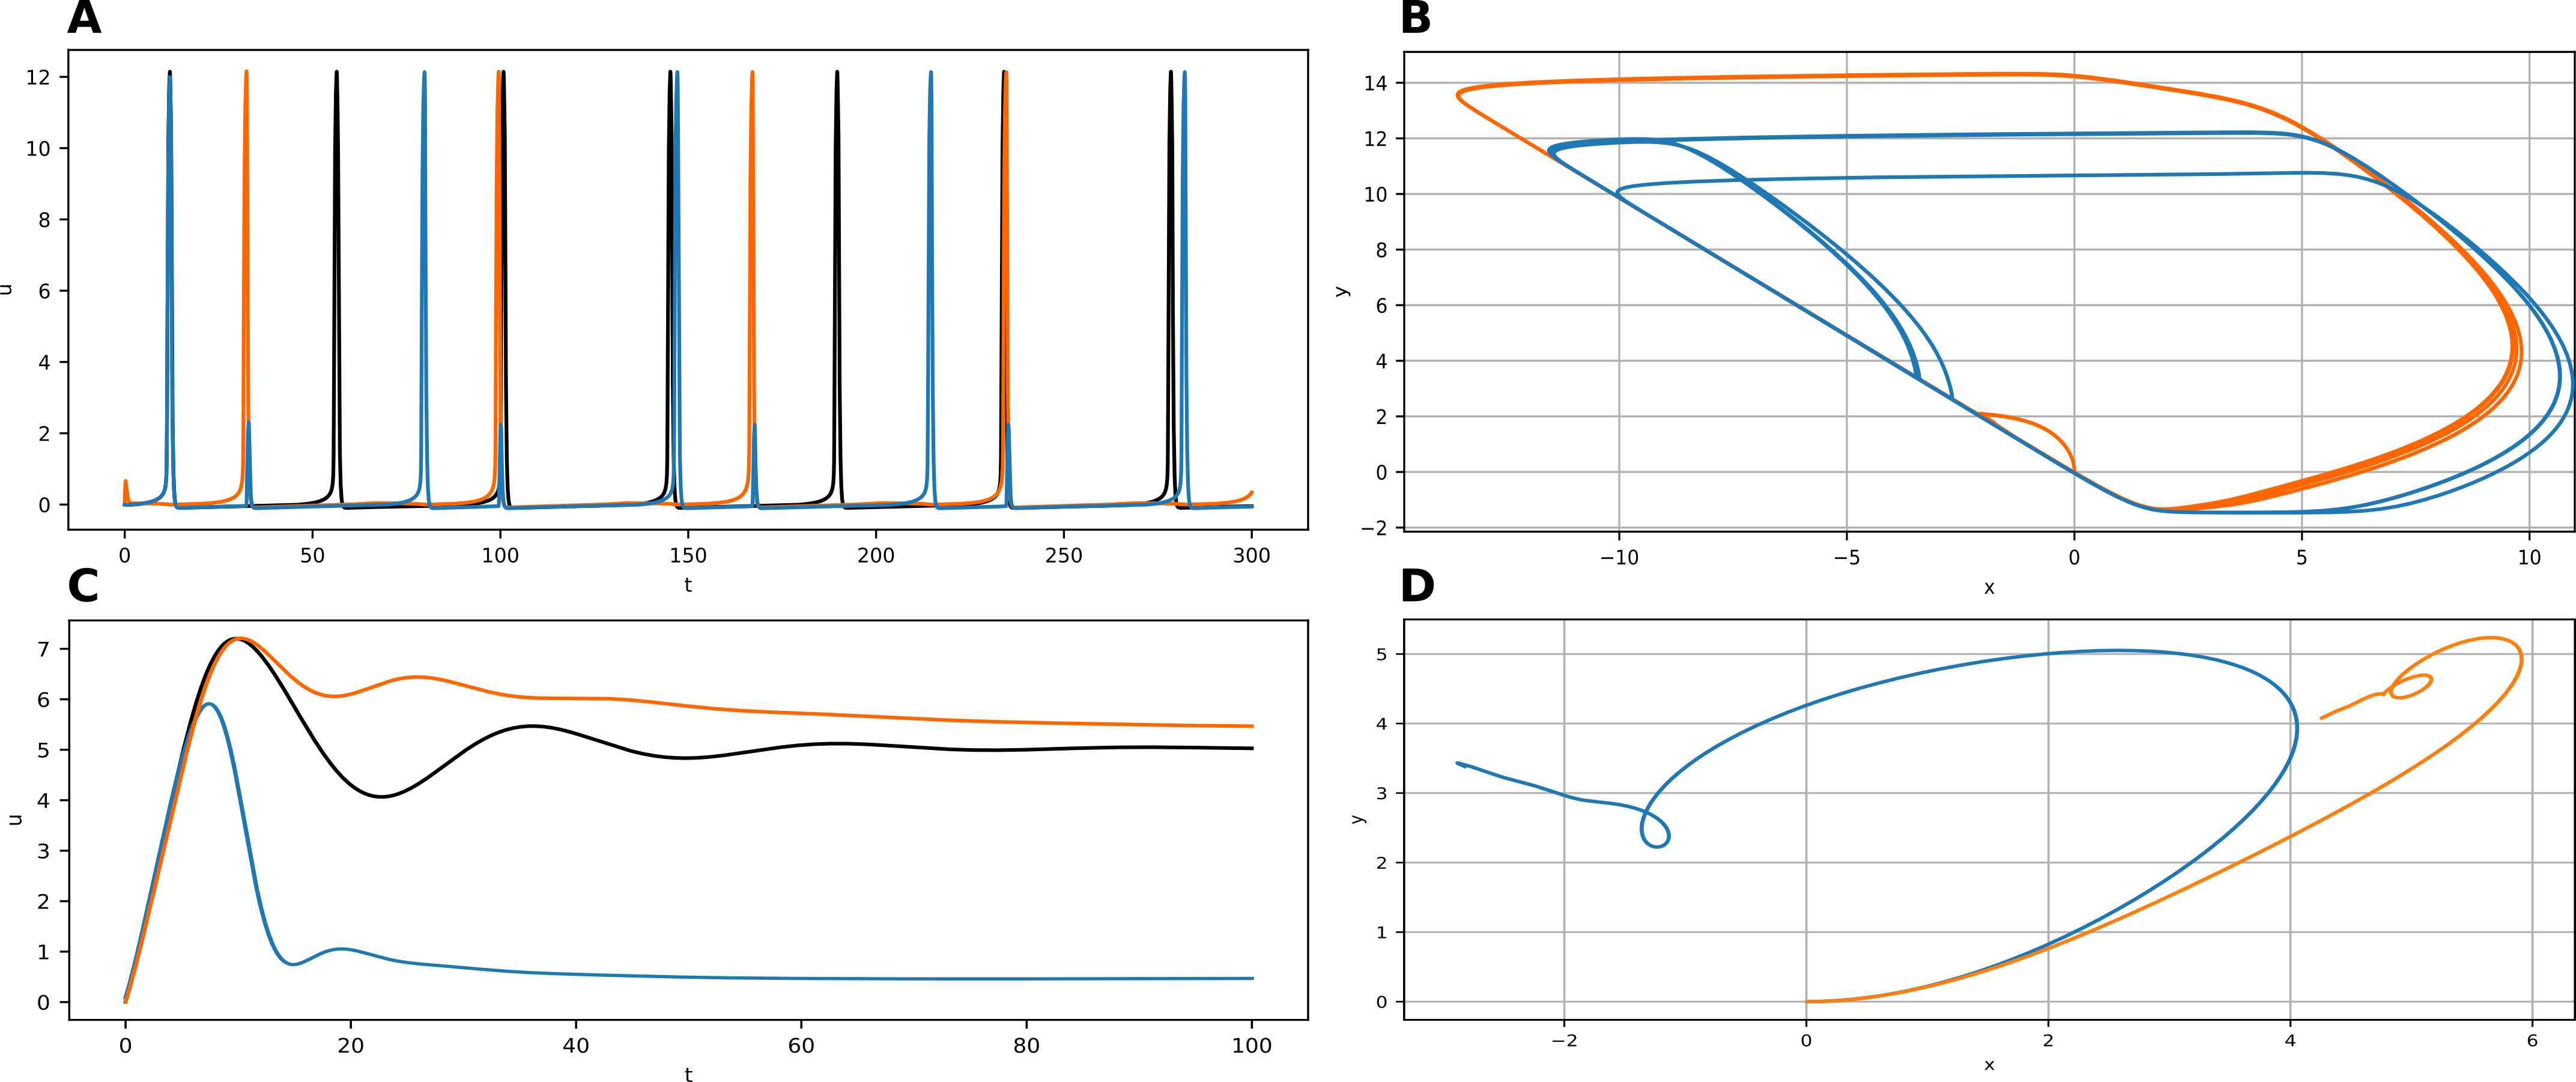
\includegraphics[width=0.9\textwidth]{../figures/graphics/network_dyn_combined.png}
\caption{Dynamics of an exc.(blue) and inh.(red) neuron mutually coupled, including additional input driving the exc. neuron. Black traces in A/C represent an isolated reference neuron driven by the same external input A/B: The network in its spiking state. C/D: Rate-encoding state, same coupling strengths.}
\end{figure}
\end{myblock}

\begin{myblock}{Conclusions}
\begin{itemize}
\item The model allows for the reproduction of a wide range of dynamical properties of spiking neurons.
\item Characteristic properties such as the spike height and width can be controlled very well by certain model parameters.
\item Good usability as a rate encoding model with a sigmoid activation function.
\item Further investigations should compare how spiking and rate network dynamics map onto each other under the same synaptic coupling.
\end{itemize}
\end{myblock}

\bibliographystyle{unsrt}
\bibliography{poster_citations}
\end{column}
\end{columns}
\end{frame}
\end{document}
